\documentclass{article}
\usepackage{graphicx, amsmath, amsthm, amssymb, mathtools, enumerate, bbm}
%\usepackage{virus}
\usepackage[a4paper, total={6in, 8in}]{geometry}
\usepackage[T1]{fontenc}
\usepackage[ngerman]{babel}


\title{Lineare Algebra II (LA) Übungsblatt 6}
\author{Erik Achilles, Alexandra Dittmar, Artur Szeczinowski}
\date{Mai 2025}




\setlength{\parindent}{0pt}


\newcommand{\NN}{\mathbb{N}}
\newcommand{\ZZ}{\mathbb{Z}}
\newcommand{\QQ}{\mathbb{Q}}
\newcommand{\RR}{\mathbb{R}}
\newcommand{\FF}{\mathbb{F}}
\newcommand{\CC}{\mathbb{C}}

\newcommand{\imp}{\mathbb{\Rightarrow}}
\newcommand{\equ}{\mathbb{\Leftrightarrow}}
\newcommand{\eq}{\mathbb{\quad = \quad}}

\DeclareMathOperator{\RRe}{Re}
\DeclareMathOperator{\IIm}{Im}
\DeclareMathOperator{\Mat}{Mat}
\DeclareMathOperator{\im}{im}
\DeclareMathOperator{\rg}{rg}
\DeclareMathOperator{\LH}{L}
\DeclareMathOperator{\Bas}{Bas}
\DeclareMathOperator{\Kern}{ker}
\DeclareMathOperator{\Abb}{Abb}
\DeclareMathOperator{\Fin}{Fin}
\DeclareMathOperator{\Konv}{Konv}
\DeclareMathOperator{\Poly}{Poly}
\DeclareMathOperator{\sign}{sign}
\DeclareMathOperator{\sgn}{sgn}
\DeclareMathOperator{\GL}{GL}
\DeclareMathOperator{\SL}{SL}
\DeclareMathOperator{\vol}{vol}

\newcommand{\limn}{\lim_{n \rightarrow \infty}}
\newcommand{\toInf}[1]{\overset{#1 \rightarrow \infty}{\longrightarrow}}

\newcommand{\movs}[2]{\overset{\text{\tiny $#1$}}{\quad #2 \quad}}
\newcommand{\tovs}[2]{\overset{\text{\tiny (#1)}}{\quad #2 \quad}}
\newcommand{\vect}[1]{\begin{pmatrix*}[c] #1 \end{pmatrix*}}
\newcommand{\sect}[1]{\begin{psmallmatrix*}[c] #1 \end{psmallmatrix*}}
\newcommand{\legs}[2]{\left(\begin{array}{#1}#2\end{array}\right)}


%% https://texblog.net/latex-archive/maths/amsmath-matrix/
\makeatletter
\renewcommand*\env@matrix[1][*\c@MaxMatrixCols c]{%
  \hskip -\arraycolsep
  \let\@ifnextchar\new@ifnextchar
  \array{#1}}
\makeatother




\begin{document}
%\maketitle
%\newpage

\section*{Aufgabe 1}
\subsection*{a) Volumina und affine Abbildungen}

Wir betrachten die Punkte
\[
  A := \vect{0\\0}, \quad
  B := \vect{2\\3}, \quad
  C := \vect{4\\-1}, \quad
  A' := \vect{-4\\-2}, \quad
  B' := \vect{8\\3}, \quad
  C' := \vect{6\\1}
  \in \RR^2.
\]
und die Dreiecke $\Delta$ mit den Eckpunkten
$A,B,C$ und $\Delta'$ mit den Eckpunkten
$A',B',C'$.
Gesucht ist eine affine Abbildung
$F: \RR^2 \to \RR^2, x \mapsto M \cdot x + b$
mit
\[
  M = \legs{cc}{ M_{11} & M_{12} \\ M_{21} & M_{22} }
  \in \Mat(2,\RR) \qquad\text{und}\qquad b \in \RR,
\]
sodass $A' = F(A)$, $B' = F(B)$ und $C' = F(C)$.
Zunächst gilt
\[
  \vect{-4\\-2} = A' = F(A) = M \cdot \vect{0\\0} + b = b
  \qquad\imp\qquad
  b = \vect{-4\\-2}.
\]
Also gilt für $B'$:
\[
  \vect{8\\3} = B' = F(B) = M \cdot \vect{2\\3} + \vect{-4\\-2}
  \qquad\imp\qquad
  M \cdot \vect{2\\3} = \vect{12\\5}.
\]
Daraus folgt
$2 \cdot M_{11} + 3 \cdot M_{12} = 12$
und
$2 \cdot M_{21} + 3 \cdot M_{22} = 5$.
Für $C'$ gilt:
\[
  \vect{6\\1} = C' = F(C) = M \cdot \vect{4\\-1} + \vect{-4\\-2}
  \qquad\imp\qquad
  M \cdot \vect{4\\-1} = \vect{10\\3}.
\]
Daraus folgt
$4 \cdot M_{11} - \cdot M_{12} = 10$
und
$4 \cdot M_{21} - \cdot M_{22} = 3$.
Daraus ergeben sich zwei LGS, die wir mit dem Gaußverfahren lösen:
\[
  \legs{cc}{2 & 3 \\ 4 & -1} \cdot \vect{M_{11} \\ M_{12}}= \vect{12 \\ 10}
  \qquad\imp\qquad
  \vect{M_{11} \\ M_{12}} = \vect{3 \\ 2}
\]
und
\[
  \legs{cc}{2 & 3 \\ 4 & -1} \cdot \vect{M_{21} \\ M_{22}}= \vect{5 \\ 3}
  \qquad\imp\qquad
  \vect{M_{21} \\ M_{22}} = \vect{1 \\ 1}.
\]
Also ist
\[
  M = \legs{cc}{3 & 2 \\ 1 & 1}.
\]
Nun gilt $\Delta' = F(\Delta)$ und daher
\[
  \vol_2(\Delta') = \vol_2(F(\Delta)) = |\det(M)| \cdot \vol_2(\Delta)
  = |(3 \cdot 1 - 2 \cdot 1)| \cdot \vol_2(\Delta) = \vol_2(\Delta).
\]




\newpage
\subsection*{b) Schiefer Zylinder}

Sei \( X \in \mathbb{K}^{n-1} \), \( \hat{b} \in \mathbb{R}^{n-1} \) und \( h > 0 \). Wir definieren den schiefen Zylinder über \( X \) durch

\[
  \hat{Z}_{\hat{b},h}(X) := \left\{
  \left( \hat{x} + \frac{s}{h} \hat{b}, s \right) \; \middle| \; \hat{x} \in X, \; s \in [0, h]
  \right\}.
\]

\subsubsection*{Beispielskizze schiefer Zylinder}
Wir verschieben $Z_2(D(1))$ mit $e_1$ und erhalten $\hat{Z}_{2,e_1}(D(1))$:
\begin{center}
  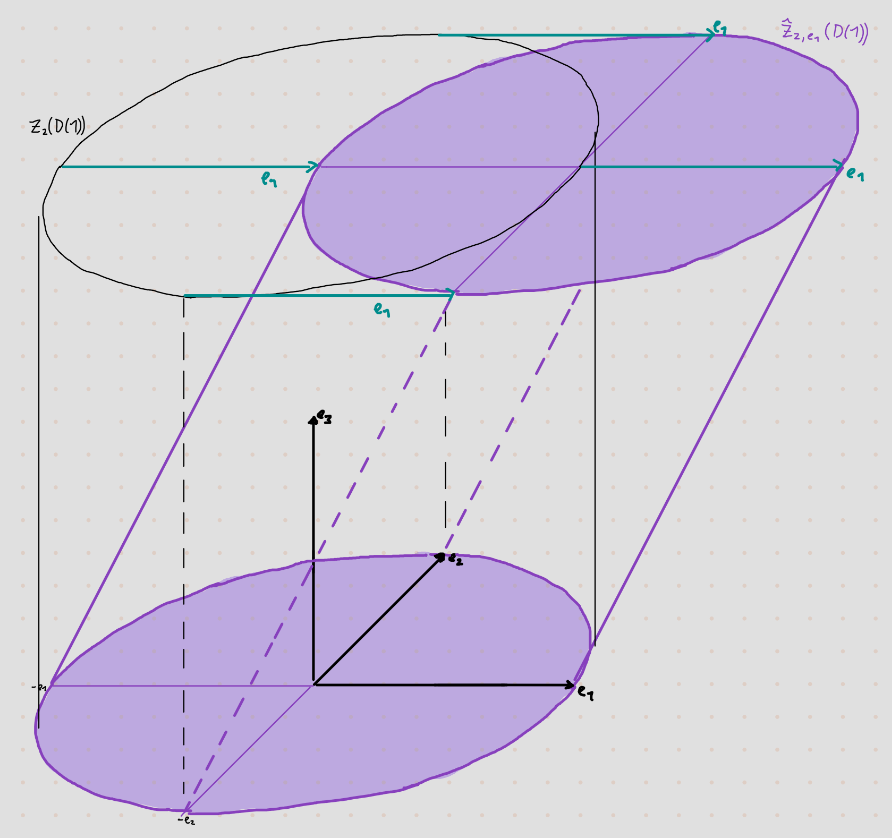
\includegraphics[width=1\textwidth]{skizze.png}
\end{center}


\newpage

\subsubsection*{Volumen des schiefen Zylinders}

Es ist $\operatorname{vol}_n \left( \hat{Z}_{\hat{b}, h}(X) \right) = h \cdot \operatorname{vol}_{n-1}(X)$.

\begin{proof}
  Der verallgemeinerte Zylinder über \( X \) ist definiert durch
  \[
    Z_h(X) := X \times [0, h] \subset \mathbb{R}^{n-1} \times \mathbb{R}.
  \]

  Wir betrachten dann die affine Abbildung
  \[
    G : Z_h(X) \rightarrow \mathbb{R}^n, \quad \begin{pmatrix} \hat{x} \\ s \end{pmatrix} \mapsto \begin{pmatrix} \hat{x} + \frac{s}{h} \hat{b} \\ s \end{pmatrix}.
  \]

  Diese Abbildung ist affin, da sie die Form
  \[
    G(x) = A \cdot x + b
    \quad \text{mit } b = 0
    \quad \text{und }  A := \begin{pmatrix}
      I_{n-1} & \frac{1}{h} \hat{b} \\
      0       & 1
    \end{pmatrix},
  \]
  hat und es gilt:
  \[
    G(x) =
    \begin{pmatrix}
      I_{n-1} & \frac{1}{h} \hat{b} \\
      0       & 1
    \end{pmatrix}
    \begin{pmatrix} \hat{x} \\ s \end{pmatrix} =
    \begin{pmatrix} \hat{x} + \frac{s}{h} \hat{b} \\ s \end{pmatrix}.
  \]

  Wir wollen nun zeigen, dass
  \[
    \operatorname{vol}_n \left( \hat{Z}_{\hat{b}, h}(X) \right) = h \cdot \operatorname{vol}_{n-1}(X).
  \]

  Wir berechnen die Determinante der Matrix \( A \):
  \[
    \det(A) = \det \begin{pmatrix} I_{n-1} & \frac{1}{h} \hat{b} \\ 0 & 1 \end{pmatrix}
    = \det(I_{n-1}) \cdot 1 - 0 \cdot \frac{1}{h} \hat{b} = 1.
  \]

  Da \( G \) eine affine Abbildung mit \( \det(G) = 1 \) ist, bleibt das Volumen beim Übergang erhalten.
  Nach \textit{Korollar 6.107} gilt daher:
  \[
    \operatorname{vol}_n \left( \hat{Z}_{\hat{b}, h}(X) \right) = |\det(G)| \cdot \operatorname{vol}_n \left( Z_h(X) \right)
    =  \operatorname{vol}_n \left( Z_h(X) \right) = h \cdot \operatorname{vol}_{n-1}(X).
    \qedhere
  \]

\end{proof}


\newpage

\section*{Aufgabe 2}

\subsection*{a)}

Für ein festes $n \in \NN$ und $s \in (0, \infty)$
sei die Abbildung
$$
  F_s: B_{R}(0) \to \RR^n , x \mapsto (s \cdot \mathbbm{1}_n) \cdot x.
$$
Für jedes $x \in B_R(0)$ gilt $\Vert x \Vert \leq R$,
also folgt für $F_s(x) = s \cdot \mathbbm{1}_n \cdot x = s \cdot x$,
dass $\Vert s \cdot x \Vert = s \cdot \Vert x \Vert \leq s \cdot R$,
und somit $F_s(x) \in B_{s\cdot R}(0)$.
Da $\det(s \cdot \mathbbm{1}_n) = s^n \neq 0$,
ist $F_s$ bijektiv.
Also ist $F_s(B_{R}(0)) = B_{s \cdot R}(0)$ und es gilt:
$$
  \vol(B_{s \cdot R}(0)) \eq
  \vol((s \cdot \mathbbm{1}_n) \cdot B_{R}(0)) \eq
  |\det(s \cdot \mathbbm{1}_n)| \cdot \vol(B_R(0)) \eq
  s^n \cdot \vol(B_R(0))
$$
Sei nun $s = \frac{19}{20}$.
Wir berechnen
\begin{align*}
  n=3: \qquad  & \frac{\vol(B_{s\cdot R}(0))}{\vol(B_R(0))}
  = s^n = \left(\frac{19}{20}\right)^3 \;\approx\; 0.86     \\
  n=10: \qquad & \frac{\vol(B_{s\cdot R}(0))}{\vol(B_R(0))}
  = s^n = \left(\frac{19}{20}\right)^{10} \;\approx\; 0.60  \\
  n=25: \qquad & \frac{\vol(B_{s\cdot R}(0))}{\vol(B_R(0))}
  = s^n = \left(\frac{19}{20}\right)^{25} \;\approx\; 0.28
\end{align*}

\subsection*{b)}
Wir bestimmen das kleinste $n \in \NN$
mit einem Schalenanteil von über $\frac{999999}{1000000}$:
\begin{align*}
              & 1 -\frac{\vol(B_{s\cdot R}(0))}{\vol(B_R(0))} = 1- \left(\frac{19}{20}\right)^n
  \geq \frac{999999}{1000000}                                                                   \\
  \equ\qquad  & \left(\frac{19}{20}\right)^n \leq \frac{1}{1000000}                             \\
  \equ\qquad  & n \geq \log_{\frac{19}{20}}\left(\frac{1}{1000000}\right) \approx 269.34        \\
  \imp \qquad & n = \lceil 269.34 \rceil = 270.
\end{align*}





\end{document}
